\chapter{随机接入网络及其建模方法}
\label{chapter2: system model}

本章旨在构建全篇论文的研究基石，对相关的理论背景、核心机制及系统模型进行系统性阐述。章节内容安排如下：首先，回顾现有的主流随机接入标准方案，重点剖析面向 5G 的概率性接入机制与面向非授权频段的载波侦听机制，在总结其技术演进路线的同时揭示现有方案的局限性，从而引出本文的研究动机；其次，深入解析连续传输机制（Successive Transmission）的基本原理，论证其在提升信道利用率方面的内在优势；接着，引入用于后续性能量化分析的核心数学工具——离散时间休假排队理论；最后，为了实现不同协议间性能的公平对比，统一构建了包含网络拓扑、信道特性及业务假设的通用系统场景模型，并定义了关键性能评估指标。

\section{典型随机接入标准方案及其演进}
\label{sec:standard_schemes}

本节从\textbf{机理分析}与\textbf{数学抽象}的视角，对现有随机接入协议的内在结构进行解构。我们不重点讨论应用场景与标准演进，而是聚焦于协议在MAC层的本质运作原理，并并建立与经典随机接入模型之间的对应关系。该抽象框架为后续连续传输机制设计（第~\ref{chapter3: SAST }、\ref{chapter4: CSMAST } 章）
以及 AI 多协议选择（第~\ref{chapter5: ai_selector} 章）提供统一理论基础。

\subsection{基于连接的5G NR随机接入过程}
\label{subsec:cba_mapping}
\begin{figure}[t]
	\centering
	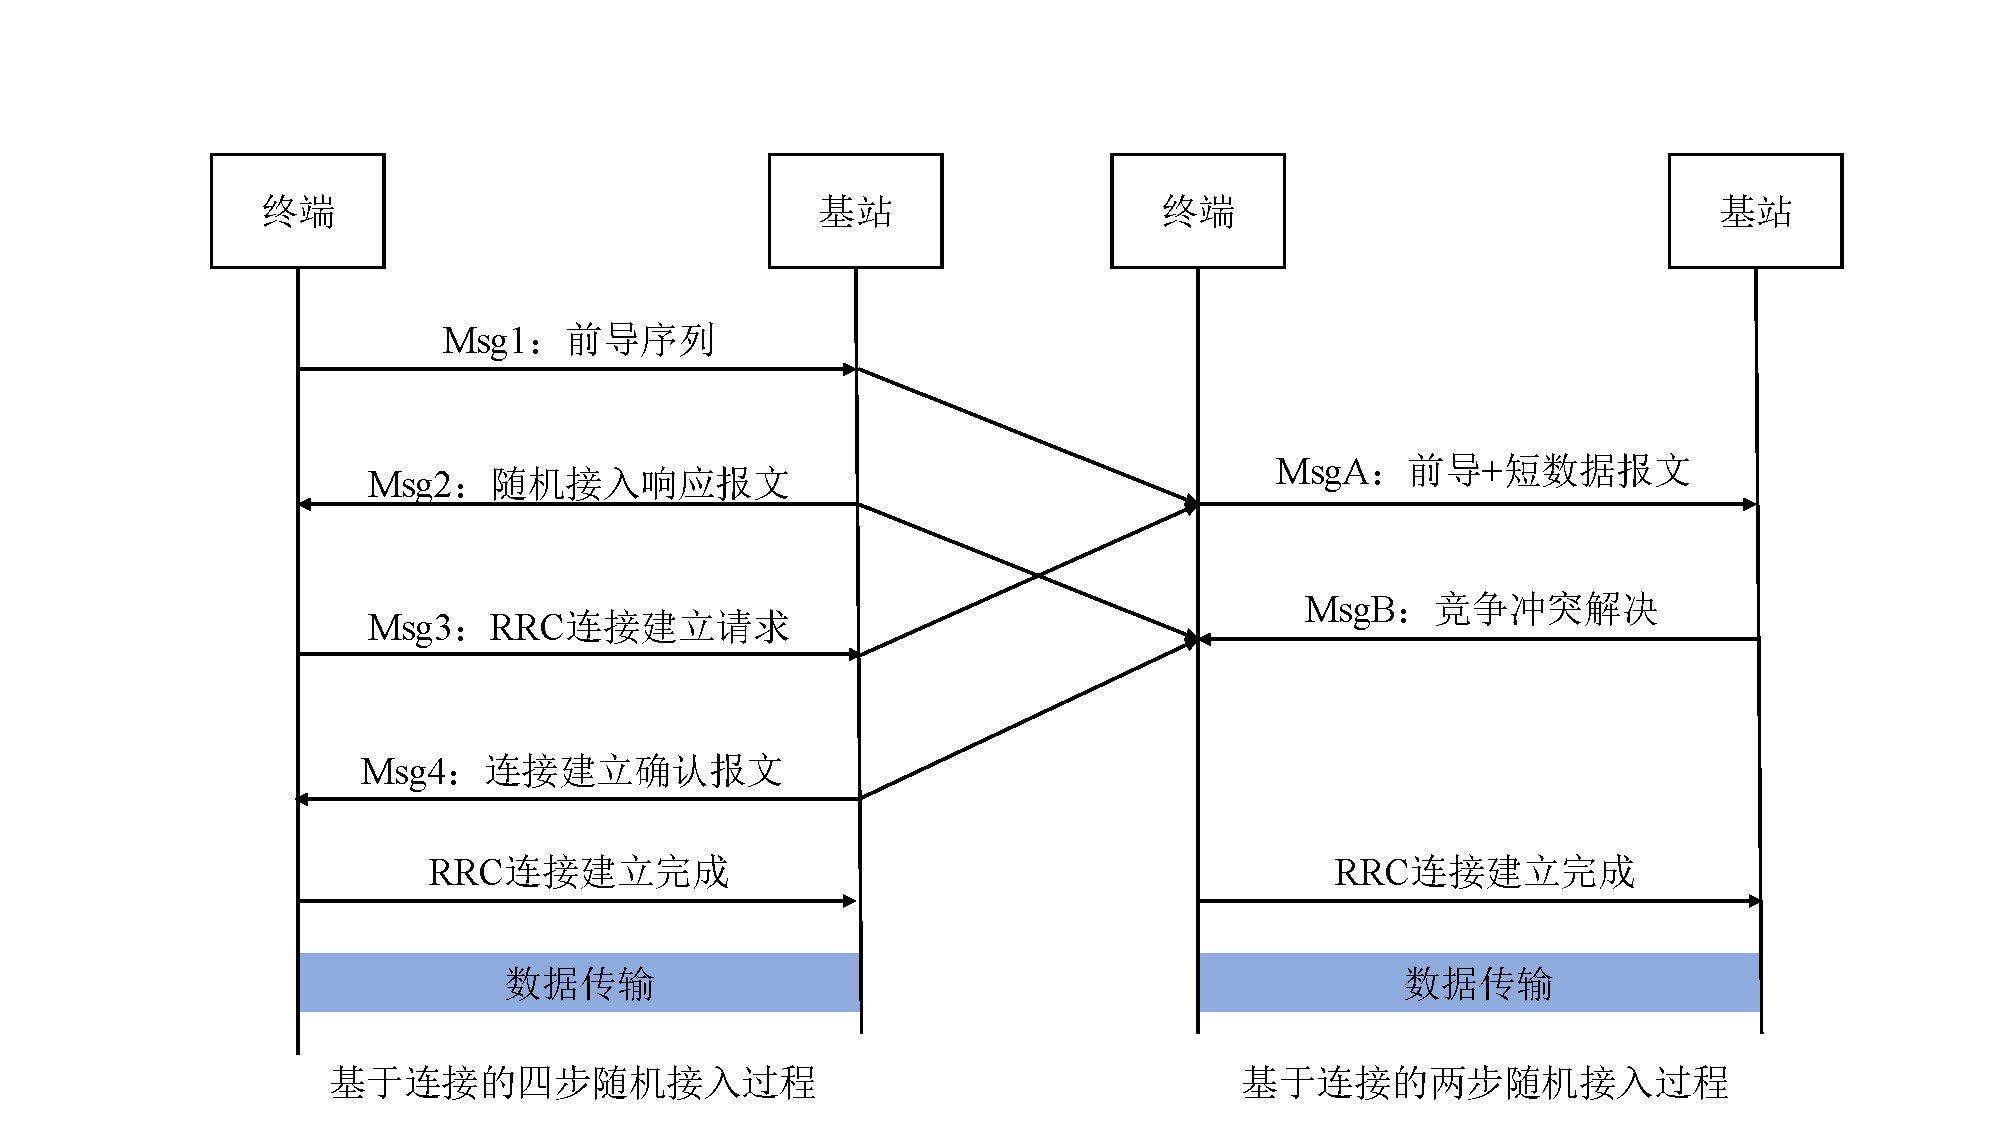
\includegraphics[width=0.95\linewidth]{figure/chap2/5G NR标准随机接入过程.pdf}
	\caption{5G NR 四步/两步标准随机接入流程示意图}
	\label{fig:cba_access}
\end{figure}

5g NR 随机接入过程，从先前的 4G LTE 随机接入过程演变而来。在 5G NR 的基于连接的数据传输模式下，终端在初始随机接入成功后，由基站分配专用无线资源，并在连接期间进行数据传输。现提出的标准方案中存在四步接入和两步接入两种流程，前者在竞争阶段包含更多的握手消息以提高可靠性，而后者则通过合并前导码与数据包来降低接入时延。两种流程图表示如\ref{fig:cba_access}所示。

从接入机理上看，无论四步还是两步，都具有明显的两阶段结构：（1）竞争建立阶段：终端通过随机接入获得资源授权；（2）独占传输阶段：终端在被分配资源上进行连续数据发送。第一阶段与 Slotted Aloha 具有相同的概率竞争特征，而第二阶段则表现为无竞争的资源独占。

因此，可将该结构抽象为一种竞争-预留模型，记为$\text{CBA}(q, M)$,其中：$q$ 为接入阶段的竞争概率；$M$ 为一次竞争成功后可连续占用的传输时隙数。当 $M=1$ 时，该模型退化为标准 Aloha；当 $M>1$ 时，竞争成本可在多个数据包之间分摊，从而提升单位数据的有效吞吐效率。
因此，5G 基于连接的数据传输机制在 MAC 层抽象上可视为 Connection-Based Aloha 的一种实现。

\subsection{面向短报文传输的5G NR随机接入机制}
\label{subsec:sdt_mapping}
\begin{figure}[t]
	\centering
	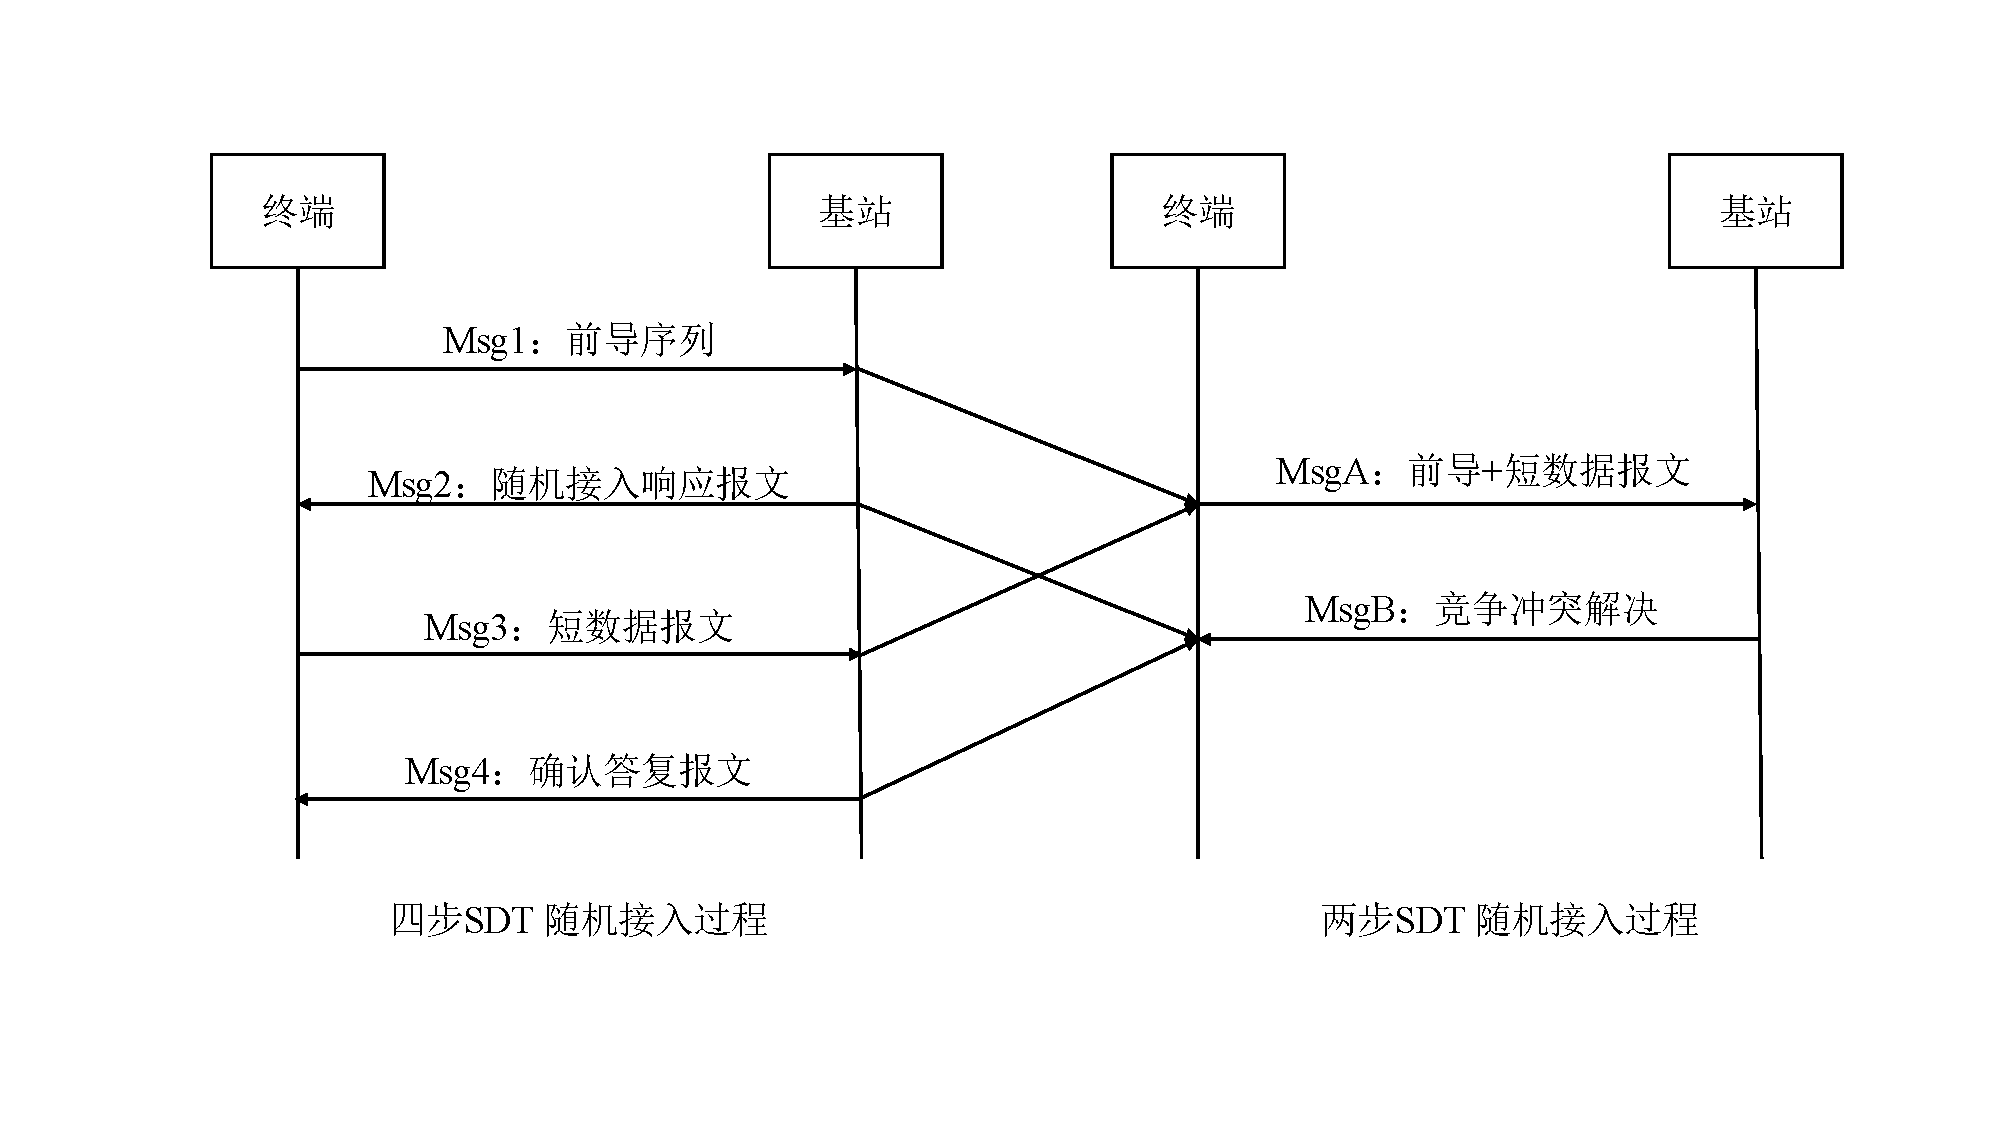
\includegraphics[width=0.95\linewidth]{figure/chap2/5G NR SDT标准随机接入过程.pdf}
	\caption{5G NR 四步/两步 SDT 标准随机接入流程示意图}
	\label{fig:sdt_access}
\end{figure}
在 5G NR 的短数据传输（Short Data Transmission, SDT）场景中，终端在无既有连接状态下，需要首先通过随机接入建立初始通信。在四步SDT标准接入方案中，终端通过发送 Msg1 前导码发起接入，在Msg3传输短报文；而在两步 SDT 标准接入方案中，终端将前导码与数据封装于 MsgA 中一并发送。
尽管信令流程存在差异，但在初始接入阶段，多个终端在离散配置的 PRACH 时隙中独立发起发送请求。两种流程图表示如\ref{fig:sdt_access} 所示。


从 MAC 层视角，每个终端在一个接入机会内仅面临两种决策：发起发送或者保持静默。
该决策可抽象为一次伯努利试验，其发送概率记为 $q \in [0,1]$。不同终端之间的发送行为在统计意义上相互独立。
因此，短报文随机接入在 MAC 抽象层面可视为一种\textbf{时隙化概率竞争机制}，其行为结构与经典的 Slotted Aloha 模型一致，也就是节点在离散时隙中以概率 $q$ 发送，
当且仅当该时隙内恰有一个节点发送时，接入成功。
因此，在不考虑物理层调制、编码等实现细节的前提下，5G 短报文随机接入的接入结构可在理论上等价映射为 Slotted Aloha。

\subsection{NR-U中基于LBT的随机接入过程}
\label{sec:csma_mapping}

在 NR-U（New Radio in Unlicensed Spectrum）场景中，终端在非授权频段发送数据前必须执行Listen-Before-Talk (LBT) 机制。这里假设设备终端已经完成初始接入过程进入到 RRC\_CONNECTED 状态，并且在后续数据传输过程中需要遵守 LBT 规则。根据 3GPP 规范\cite{3gpp38213}，LBT 可分为四种类型（Cat 1–4），其复杂程度与竞争控制能力逐级增强。
\begin{itemize}
    \item Cat 1：无需 LBT；
    \item Cat 2：固定持续时间的信道检测；
    \item Cat 3：随机退避但无指数扩展；
    \item Cat 4：带指数退避的随机退避机制。
\end{itemize}
其中，Cat 4 引入了随机退避与竞争窗口扩展，其结构最接近经典 CSMA/CA。因此，本节重点分析 Cat 4 机制的流程如图\ref{fig:lbt_process}所示，即

\begin{figure}[t]
\centering
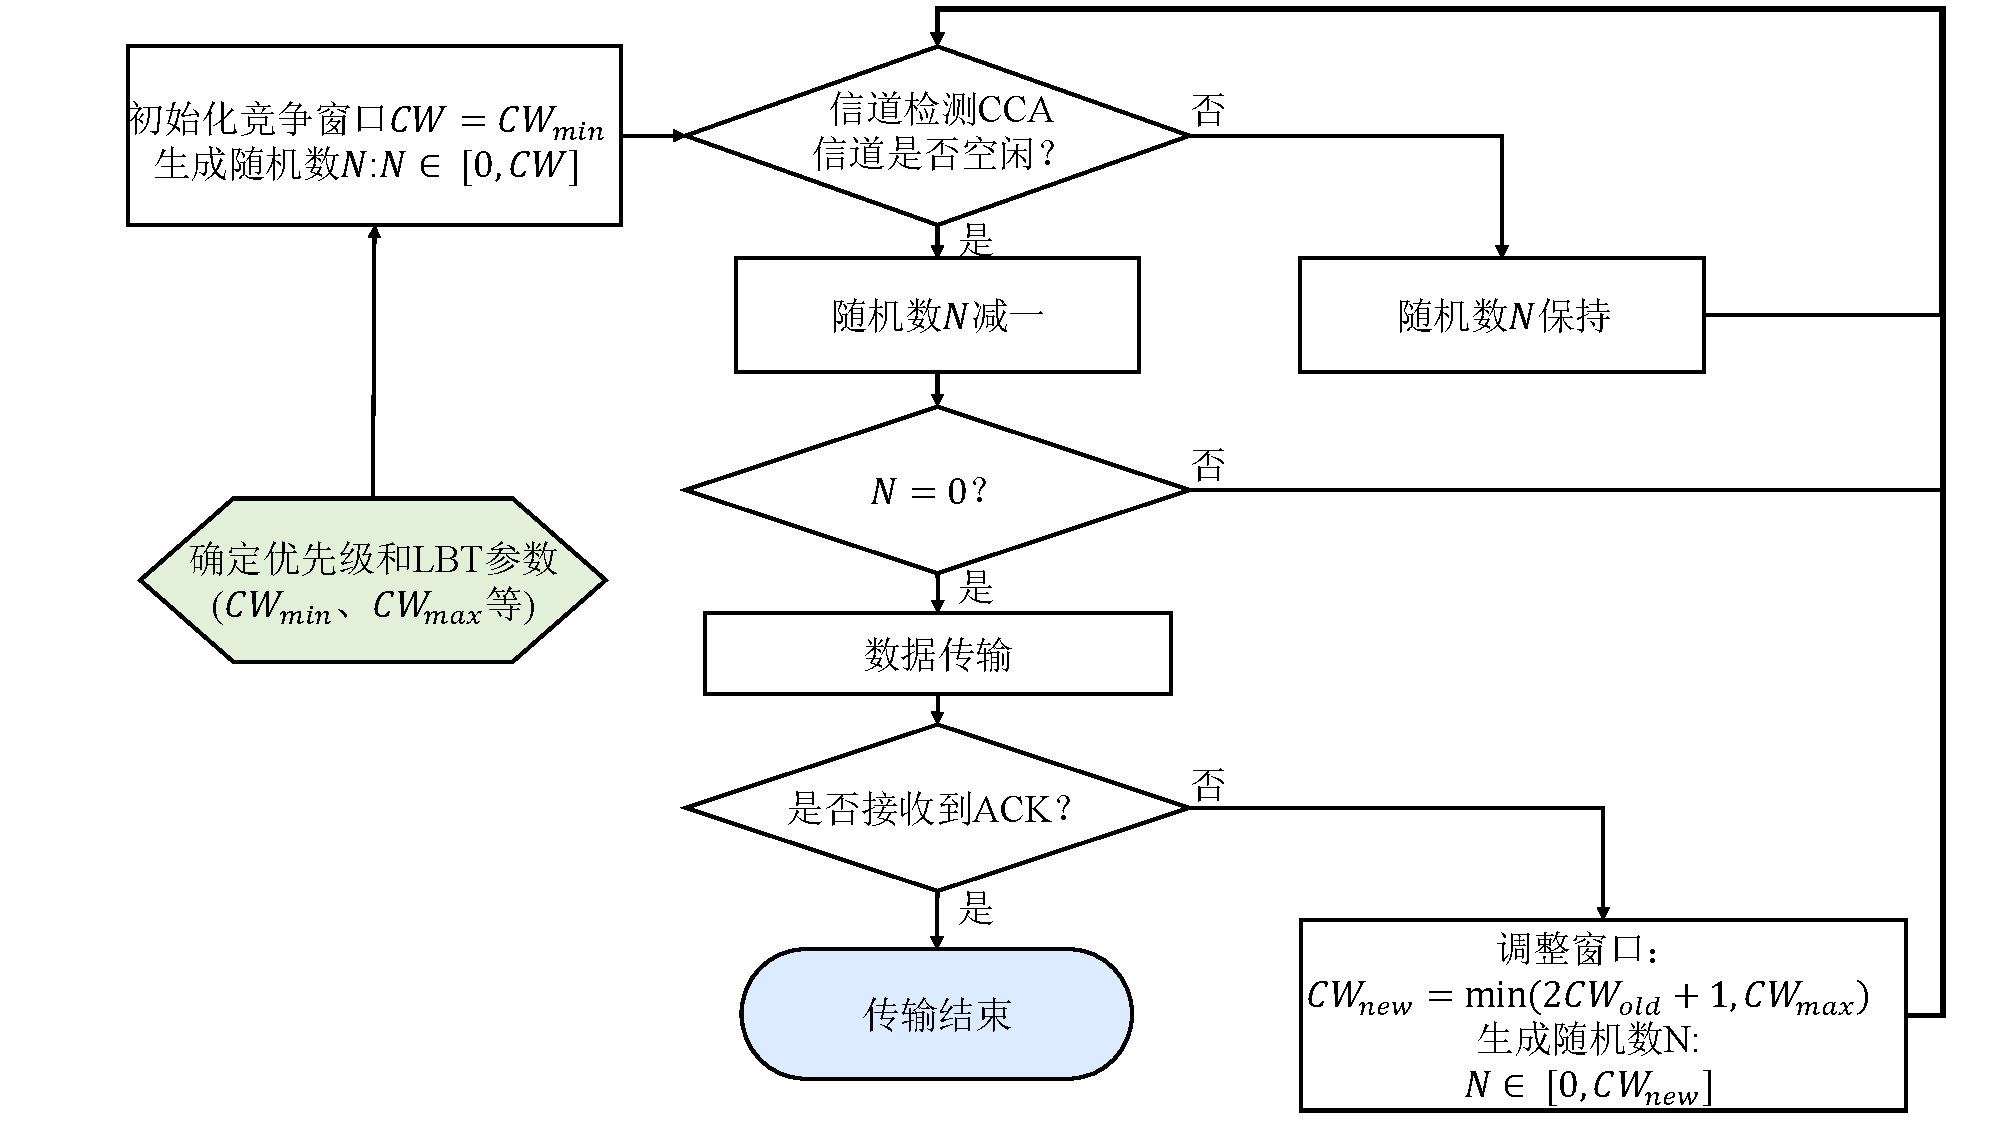
\includegraphics[width=0.9\linewidth]{figure/chap2/5G NR标准LBT过程.pdf}
\caption{NR-U中基于LBT的随机接入流程}
\label{fig:lbt_process}
\end{figure}

\begin{enumerate}[label=\textbf{步骤 \arabic*：}, leftmargin=*, itemsep=1ex]

    \item \textbf{确定信道接入优先级与参数} \\  
    终端在发起传输前，根据业务 QoS 要求选择信道接入优先级类别（Channel Access Priority Class, CAPC）。    每个 CAPC 对应一组预定义的 LBT 参数，包括延迟持续时间参数 $m_p$、竞争窗口最小值 $CW_{\min}$、最大值 $CW_{\max}$，以及最大信道占用时间（Maximum Channel Occupancy Time, MCOT）。
    MCOT 受监管约束限制，用于保证与其他系统的公平共存。

    \item \textbf{竞争窗口更新与退避计数初始化} \\  
    终端根据上一轮传输结果更新竞争窗口 $CW$：
    \begin{itemize}
        \item 若传输成功或为初始传输，则 $CW = CW_{\min}$；
        \item 若传输被判定为失败（例如未收到 HARQ-ACK 或检测到冲突），则
        $CW \leftarrow \min(2CW+1, CW_{\max})$。
    \end{itemize}
    随后在整数区间 $[0, CW]$ 内均匀随机选择退避计数值 $N$。
	
    \item \textbf{执行延迟持续时间（Defer Duration）检测} \\  
    在开始退避计数前，终端必须检测信道在连续时间$T_d = 16\mu s + m_p \times 9\mu s$
    内保持空闲（典型 5 GHz 配置）。若期间检测到信道忙，则需等待信道重新空闲，并重新执行完整的延迟持续时间检测。

    \item \textbf{退避计数与 CCA 时隙监听} \\  
    终端在 $9\mu s$ 的 CCA 时隙上执行退避计数：
    \begin{itemize}
        \item 若信道空闲，则 $N \leftarrow N-1$；
        \item 若信道忙，则冻结计数器，
        待信道重新空闲并重新满足步骤 3 的延迟持续时间要求后恢复倒计时。
    \end{itemize}
    当 $N=0$ 时，终端获得发送机会。

    \item \textbf{数据发送与 MCOT 约束} \\  
    终端在获得信道后进行数据传输，
    传输持续时间不得超过该 CAPC 对应的 $T_{mcot,p}$。
    传输结束后，
    根据成功或失败结果更新 $CW$，
    为下一次接入做准备。
\end{enumerate}

从接入机制的本质出发，Type 4 LBT 与经典 CSMA/CA 在 MAC 层具有一一对应的竞争逻辑：二者均遵循“先侦听、后发送”的信道占用原则，均通过随机退避计数分散并发发送时机，并在失败后通过竞争窗口扩展抑制后续冲突概率。因而，在以时隙化 CCA、理想碰撞信道和饱和/非饱和队列业务为前提的理论分析框架下，NR-U 的 LBT 过程可等效抽象为 CSMA 型随机接入网络。该抽象保留了影响吞吐量、时延与公平性的主要竞争行为，同时忽略物理层调制、频谱监管细节与跨系统共存策略等次要差异，因此可作为后续 CSMA 网络建模与性能推导的合理基础。

\section{连续传输机制的基本原理}
\label{sec:continuous_transmission_principle}



传统随机接入协议（如 Aloha 与 CSMA）通常采用一次竞争、发送一个数据包的工作方式：节点每完成一次发送后都需释放信道，并重新进入竞争或退避过程。该机制在中高负载下会反复消耗竞争时隙，使大量时间开销停留在侦听、退避与握手环节而非有效载荷传输。为降低这部分重复开销，本文引入连续传输（Successive Transmission, ST）机制：节点一旦竞争成功并完成队首分组发送，可在满足协议约束的条件下继续发送后续缓存分组，直到队列清空或触发释放条件，再重新进入竞争过程。

如图\ref{fig:ra_vs_st} 所示，传统机制下每个数据包通常对应一次独立竞争，竞争开销与数据包数量近似线性增长；而在 ST 机制下，一次竞争成功可支撑多个数据包连续发送，使竞争开销由“按包重复发生”转变为“按轮次分摊”。因此，ST 的核心增益在于降低单位数据包的平均竞争开销（Contention Overhead），并在不改变随机接入基本竞争框架的前提下提升有效信道利用率与系统吞吐效率。
\begin{figure}[t]
	\centering
	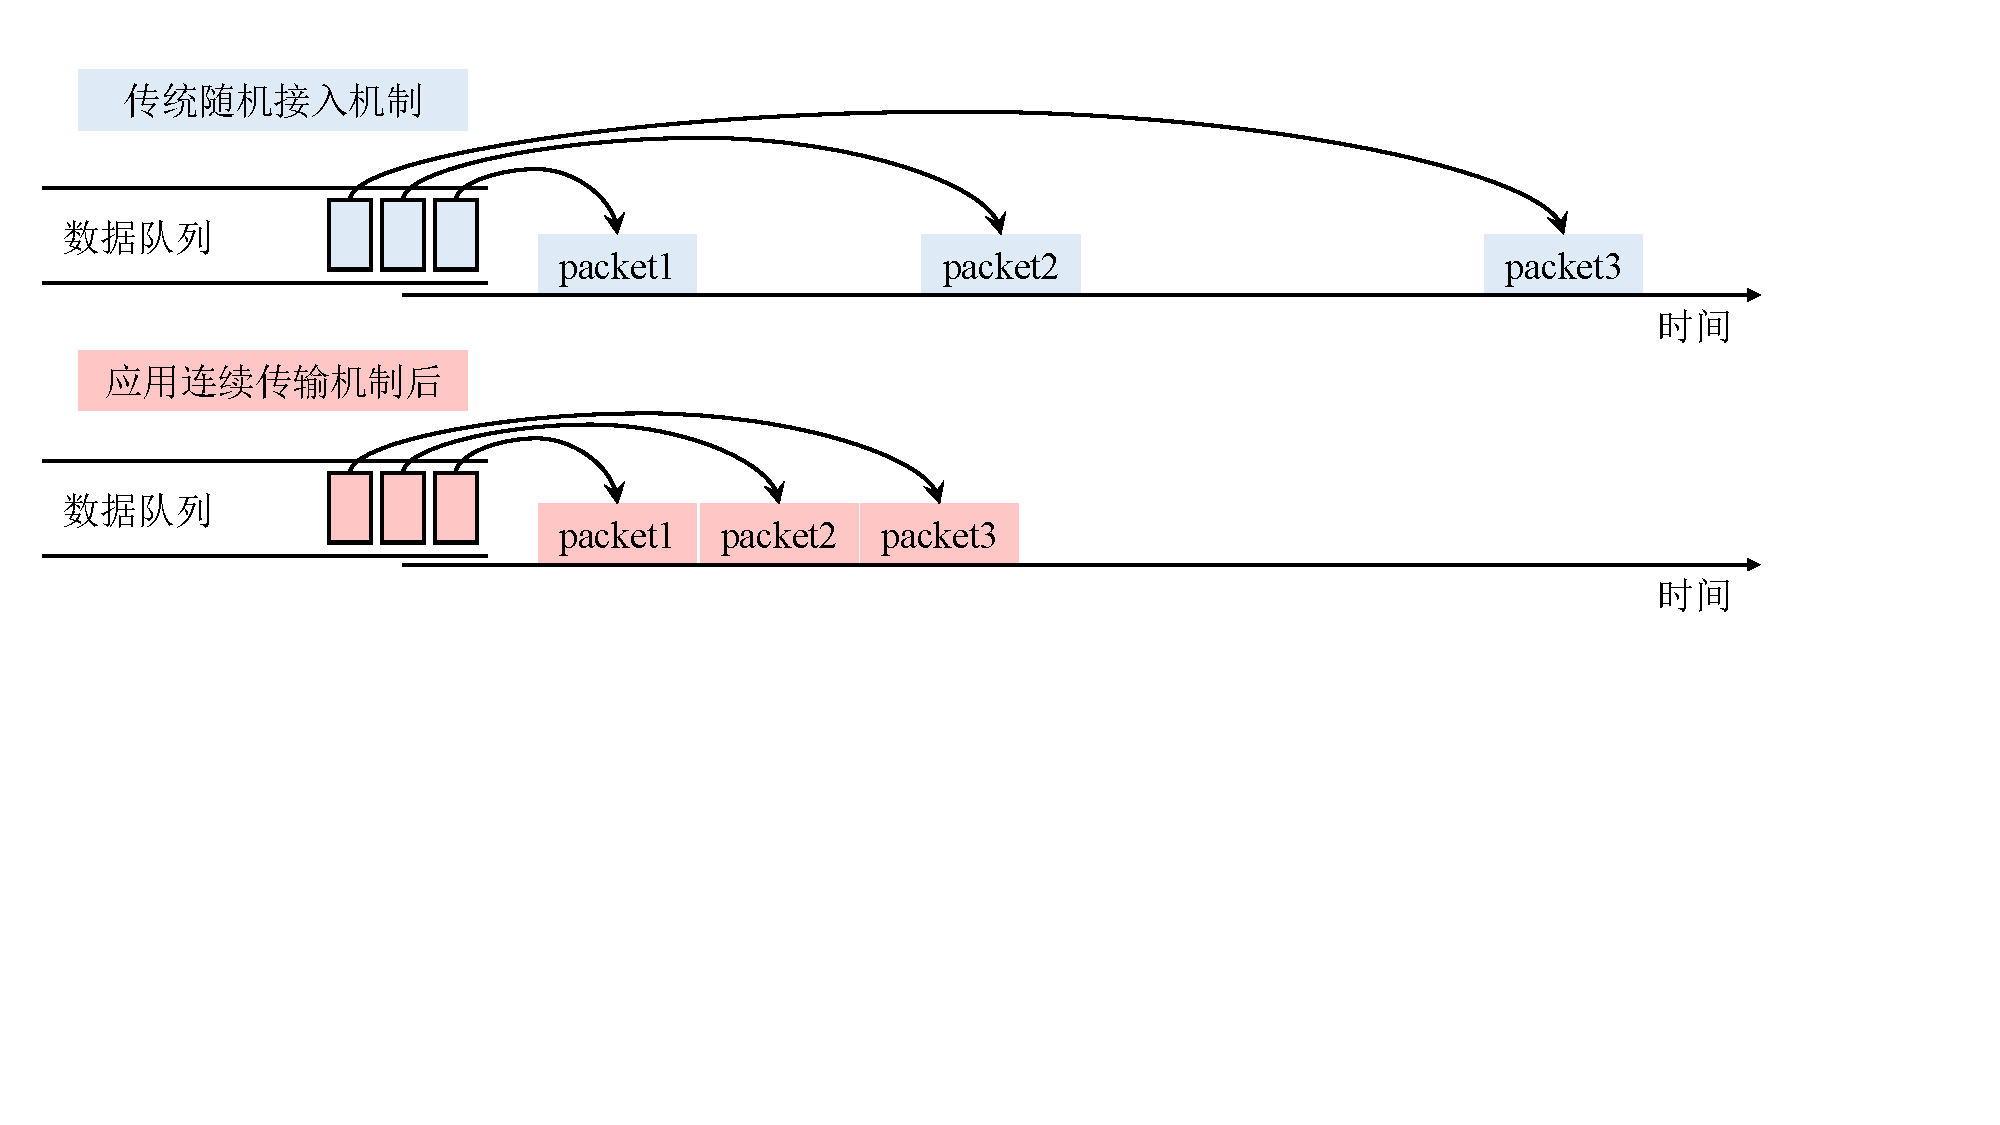
\includegraphics[width=0.95\linewidth]{figure/chap2/连续传输机制对比图.pdf}
	\caption{传统随机接入与连续传输机制的对比图}
	\label{fig:ra_vs_st}
\end{figure}
\section{通用系统场景与模型假设}
\label{sec:general_system_model}


为构建具有普适性与可扩展性的理论分析框架，并为后续章节中不同接入机制（SAST 与 CSMAST）的性能比较提供统一分析基准，本文首先建立一个抽象化的上行随机接入网络系统模型。在保证物理拓扑结构一致性的前提下，通过对节点行为机制进行差异化建模，实现对多种接入范式的统一刻画与对比分析。

本章节考虑一个包含 $n$ 个同质终端节点（User Equipment, UE）和一个中心基站（Base Station, BS，亦作为统一接收机）的上行通用无线随机接入系统，如图~\ref{fig:system_model} 所示。所有节点通过共享无线信道向同一接收机发送数据，接收机负责信号接收、译码与反馈。系统中仅接收机设计接收结构，而节点之间不存在显式协调或直接通信机制。
\begin{figure}[t]
	\centering
	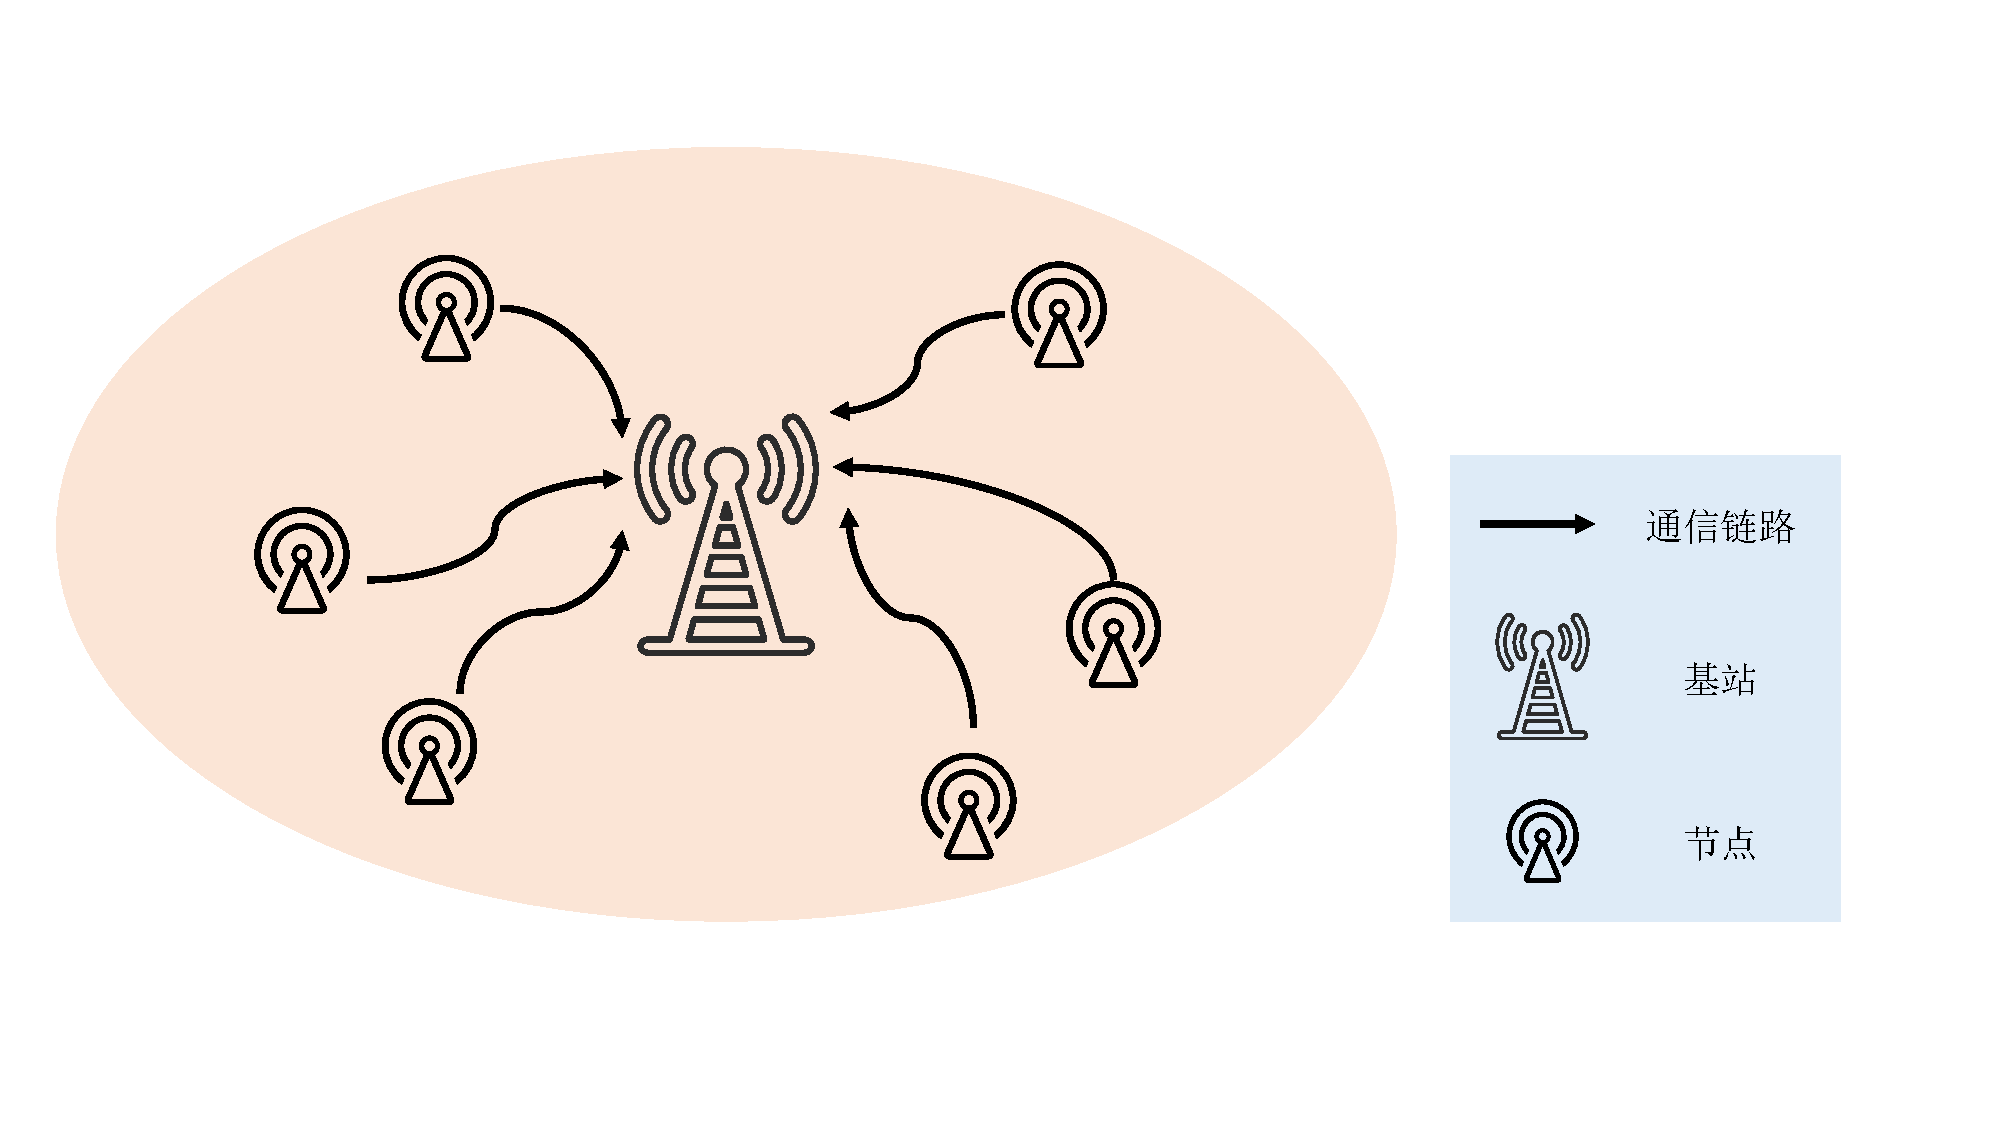
\includegraphics[width=0.9\linewidth]{figure/chap2/通用系统场景.pdf}
	\caption{通用系统场景示意图}
	\label{fig:system_model}
\end{figure}

需要特别说明的是，尽管后续各章节的分析重点不同，但“接收机—节点”物理拓扑关系在全文中保持一致。不同章节之间的差异主要体现在节点侧接入策略与控制逻辑的设计，而非系统结构本身的改变。具体而言：

\begin{itemize}
	\item 在第~\ref{chapter3: SAST }章中，基站主要承担集中接收与反馈功能，终端节点的行为建模侧重于概率发送与连续传输的传输策略，系统分析聚焦于基于连续传输的时隙 ALOHA 机制的性能刻画；
	
	\item 在第~\ref{chapter4: CSMAST }章中，基站仍作为统一接收实体，而终端节点行为进一步扩展为“侦听—退避—发送”的竞争式接入过程，系统模型引入载波监听机制和连续传输，用以刻画 CSMAST 协议的动态行为和性能分析；
	
	\item 在第~\ref{chapter5: ai_selector}章中，在保持统一拓扑结构不变的前提下，研究重点转向不同协议与参数组合下的性能评估与接入协议智能切换机制。此时节点配备有多重接入协议策略，其具体接入行为被抽象为可切换的策略集合，分析核心从单一接入协议到多接入协议策略集合的性能。
\end{itemize}

在上述通用系统场景框架下，具体系统假设如下：

\begin{itemize}
	\item \textbf{网络拓扑与流量模型}：网络由 $n$ 个统计特性相同的同质节点组成。各节点的数据包到达过程独立且同分布（i.i.d.）。
	
	为了便于第\ref{chapter3: SAST }、\ref{chapter4: CSMAST }章的排队论解析推导，本文在\textbf{理论分析模型}中假设各节点的包到达过程均服从参数为 $\lambda$ （单位：包/时隙）的伯努利过程，即每个节点在每个时隙有新数据包到达的概率为 $\lambda$，且不同时隙的到达事件相互独立，因而系统的总到达率为 $\hat{\lambda} = n\lambda$。这一简化假设使得系统动态可精确刻画为离散时间马尔可夫链，便于应用休假排队理论进行闭式求解。
	
	然而，现实通信场景中的到达过程通常具有显著的非平稳性与多尺度统计特征。为与第\ref{chapter5: ai_selector}章保持一致，本文在仿真与业务建模中采用统一流量特征向量
	$\mathbf{x}_{\text{traffic}}=[\hat{\lambda},\ \mathrm{BI}_{\mathrm{net}},\ \mathrm{BI}_{\mathrm{node}},\ \Psi_{\mathrm{net}},\ \Psi_{\mathrm{node}}]^{\top}$，
	其中网络突发度与网络周期性强度分别定义为
	$\mathrm{BI}_{\mathrm{net}}=\frac{\mathrm{ID}_{\mathrm{net}}-1}{\mathrm{ID}_{\mathrm{net}}+1}$、
	$\mathrm{ID}_{\mathrm{net}}=\frac{\mathrm{Var}(X(t))}{\mathbb{E}[X(t)]}$，以及
	$\Psi_{\mathrm{net}}=\max_{1\le\tau\le\tau_{\max}}\frac{R(\tau)}{R(0)}$。
	在该定义下，本文采用与第\ref{chapter5: ai_selector}章一致的三类典型流量形态：
	\begin{itemize}
		\item \textbf{均匀到达场景（U）}：$\mathrm{BI}_{\mathrm{net}}\approx 0$ 且 $\Psi_{\mathrm{net}}\approx 0$，对应近似泊松到达；
		\item \textbf{突发到达场景（B）}：$\mathrm{BI}_{\mathrm{net}}\in[0.3,0.7]$ 且 $\Psi_{\mathrm{net}}\in[0,0.2]$，采用 MMPP/批量到达过程刻画事件驱动型集中上报；
		\item \textbf{周期到达场景（P）}：$\mathrm{BI}_{\mathrm{net}}\in[-0.5,-0.2]$ 且 $\Psi_{\mathrm{net}}\in[0.6,0.9]$，刻画规则采样或同步上报业务。
	\end{itemize}
	
	上述流量特征的完整定义与计算公式见第\ref{chapter5: ai_selector}章表~\ref{tab:traffic_feature_def}，具体参数配置与采样策略见该章仿真实验部分。
	
	\item \textbf{时隙结构与同步}：系统采用离散时间模型，时间轴被划分为连续且等长的时隙（Time Slot）。时隙长度被标准化为传输一个固定长度数据包所需的时间。系统假定所有节点保持严格的时钟同步，因此所有数据包的传输只能在每个时隙的起始时刻发起。
	
	\item \textbf{信道模型}：假设信道为理想无噪声信道，采用标准的碰撞信道模型（Collision Model）。当且仅当一个时隙内只有一个节点进行传输时，接收机才能成功解码数据包；若多个节点在同一时隙并发传输，则发生信号叠加导致碰撞，所有涉及的数据包均传输失败且无法恢复。
	
	\item \textbf{反馈机制}：假设基站提供完美且即时的反馈。节点在每个传输时隙结束时，能够立即通过 ACK（确认）或 NACK（否定确认）信令获知该次传输是否成功。分析中忽略反馈信道的传输错误及传播延迟。
	
	\item \textbf{数据包与信令开销}：假设系统中传输的所有数据包具有固定的长度，且完整占用一个时隙。相比之下，控制信令（如 ACK/NACK）的数据量极小，其传输时间在分析中被视为瞬时完成，或已包含在时隙的保护间隔（Guard Interval）内，不额外占用数据传输资源。
	
	\item \textbf{缓存队列与网络状态}：每个节点配备容量无限大的缓冲区（Infinite Buffer），数据包在缓冲区中遵循先进先出（FIFO）原则。在此假设下，数据包不会因缓存溢出而丢失，但可能会在队列中积压。根据节点缓存的积压情况，我们将网络运行状态划分为两类用于后续分析：
	\begin{itemize}
		\item \textbf{饱和状态（Saturated State）}：假设节点缓存始终非空（即 $p_{ne}=1$），节点始终有数据包待传。此状态用于推导系统的理论吞吐量极限。
		\item \textbf{非饱和状态（Unsaturated State）}：节点缓存可能为空（即 $p_{ne} < 1$）。此状态更符合实际流量场景，用于评估系统的稳态时延与实际吞吐量。
	\end{itemize}
\end{itemize}

基于上述通用假设，后续章节将在统一场景下展开递进分析：第~\ref{chapter3: SAST }章聚焦 SAST 机制下 Aloha 型接入的吞吐量与时延等性能特性，第~\ref{chapter4: CSMAST }章分析 CSMAST 机制下的性能边界；在此基础上，第~\ref{chapter5: ai_selector}章进一步面向多业务与动态负载环境，综合吞吐量、时延、公平性与信令开销等指标，研究多协议智能切换与参数自适应优化问题。

\section{基于休假排队理论的分析方法}
\label{sec:vacation_queuing_theory}

在引入连续传输机制后，节点与信道状态呈现出显著的“服务—休假”交替特征：当节点竞争成功并占用信道时，系统进入忙期；当节点因退避、碰撞重传或队列暂空而未进行有效传输时，系统进入休假期。该过程具有明显的循环更新结构，使得仅依赖低维状态转移的传统马尔可夫描述在表达能力与可解性之间面临权衡。为此，本文采用离散时间休假排队理论（Discrete-time Vacation Queuing Theory）作为后续理论推导的统一分析框架。

在该框架中，复杂竞争行为被重构为忙期长度与休假期长度两类随机过程的耦合分析问题。前者刻画一次成功接入后连续服务的持续能力，后者刻画节点在非服务阶段经历的等待、退避与重试代价。基于这一分解，系统关键性能可由可解释的统计量统一表征：忙期主导有效数据服务能力，休假期主导竞争开销与等待时延。

进一步地，本文从“信道视角”与“节点视角”两个层面开展分析。信道视角关注聚合流量下忙期—休假期交替规律，以推导系统吞吐量及其稳定工作区间；节点视角关注单节点队列在休假期内的积压增长与忙期内的服务消减，结合概率生成函数（PGF）及其变换性质求取队列稳态分布，并据此利用 Little 定律得到平均时延表达式。由此建立的分析路径可在统一数学框架下同时覆盖 Aloha 与 CSMA 两类机制，并为第~\ref{chapter3: SAST }章、第~\ref{chapter4: CSMAST }章及第~\ref{chapter5: ai_selector}章中的性能推导、对比与策略优化提供一致且可复用的理论基础。

\section{关键性能指标定义}
\label{sec:performance_metrics}

为了全面评估所提机制的有效性，并与现有标准方案进行公平对比，本章统一定义以下关键性能指标，涵盖效率、时延、公平性与开销四个维度。

\subsection{吞吐量指标}

吞吐量是衡量系统有效传输能力的核心指标,本文细分为接入吞吐量与数据吞吐量两类：

\begin{itemize}
	\item \textbf{接入吞吐量（Access Throughput, $S_a$）}：定义为单位时间（时隙）内成功传输的队首数据包（Head-of-Line Packet）或接入请求的平均数量，单位为包/时隙。该指标反映了系统处理并发接入请求的能力，对应于信道视角下的成功接入事件率。在理论分析中，接入吞吐量可通过竞争成功概率与节点非空概率的乘积计算：
	\begin{equation}
	S_a = n \cdot p_{tx} \cdot (1 - p_{tx})^{n-1} \cdot p_{ne}
	\end{equation}
	其中 $n$ 为节点数，$p_{tx}$ 为发送概率，$p_{ne}$ 为节点非空概率。
	
	\item \textbf{数据吞吐量（Data Throughput, $S_d$）}：定义为单位时间内信道成功传输的所有数据包（包含连续传输的后续包）的平均数量，单位为包/时隙。该指标衡量系统的有效负载传输效率。对于引入连续传输的系统，数据吞吐量显著高于接入吞吐量，两者之比反映了连续传输的增益：
	\begin{equation}
	\text{Throughput Gain} = \frac{S_d}{S_a}
	\end{equation}
\end{itemize}

\subsection{时延指标}

时延直接影响用户体验与服务质量，本文区分接入时延与端到端数据包时延：

\begin{itemize}
	\item \textbf{接入时延（Access Delay, $D_a$）}：定义为一个数据包从到达队首（成为HoL包）开始，到其成功被基站接收所经历的时间，单位为时隙。该指标主要体现竞争接入的等待成本，包含碰撞重传与退避等待时间。在休假排队模型中，接入时延等于休假期长度的期望值。
	
	\item \textbf{数据包时延（Packet Delay, $D_p$）}：定义为数据包从生成时刻进入缓存队列，直到被成功传输完毕离开系统的全过程时延，单位为时隙。该指标包含排队等待时间（队列中排在该包前面的所有包的服务时间）与接入服务时间（该包自身的接入与传输时间），直接反映端到端用户体验。根据Little定律，平均数据包时延可表示为：
	\begin{equation}
	D_p = \frac{E[Q]}{\lambda_{eff}}
	\end{equation}
	其中 $E[Q]$ 为平均队列长度，$\lambda_{eff}$ 为有效到达率。
\end{itemize}

\subsection{公平性指标}

在多用户竞争环境中，资源分配的公平性直接影响系统的稳定性与用户满意度。本文采用Jain公平性指数（Jain's Fairness Index, JFI）作为统一的公平性度量：

\begin{equation}
\text{JFI} = \frac{\left(\sum_{i=1}^{n} x_i\right)^2}{n \cdot \sum_{i=1}^{n} x_i^2}
\end{equation}

其中 $x_i$ 表示第 $i$ 个节点在观测时间窗口内获得的资源份额（可以是成功传输的数据包数量、占用的时隙数、或获得的吞吐量）。JFI的取值范围为 $[1/n, 1]$，其中 $1/n$ 表示最不公平情况（仅一个节点占用全部资源），$1$ 表示完全公平（所有节点获得相同资源）。

在本文的分析中，我们特别关注\textbf{短期公平性（Short-term Fairness）}，即在数十至数百个时隙的观测窗口内的资源分配公平性。这是因为：\textbf{（1）}连续传输机制允许单个节点连续占用信道，可能导致短期内的不公平现象；\textbf{（2）}实时业务（如VoIP、视频流）对短期时延抖动敏感，长期统计公平性无法反映瞬时服务质量；\textbf{（3）}短期公平性能够捕捉协议在动态流量变化下的瞬态行为。第\ref{chapter4: CSMAST }章和第\ref{chapter5: ai_selector}章将采用滑动窗口法计算不同时间尺度下的JFI，以评估SAST与CSMAST机制在公平性方面的权衡。

\subsection{信令开销指标}

控制信令开销是随机接入系统的重要成本，直接影响能量效率与频谱利用率。本文统一采用以下度量方式：

\begin{itemize}
	\item \textbf{信令吞吐比（Signaling-to-Throughput Ratio, STR）}：定义为每成功传输一个有效数据包所需消耗的平均信令比特数，单位为比特/包。对于标准随机接入方案，信令包括前导码（Preamble）、握手消息（Handshake）、反馈信令（ACK/NACK）等。STR越低，说明系统的信令效率越高。在第\ref{chapter3: SAST }章的理论分析中，STR可表示为：
	\begin{equation}
	\text{STR} = \frac{C_{pre} + C_{hs} + C_{ack} \cdot E[N_{tx}]}{L_{data}}
	\end{equation}
	其中 $C_{pre}$、$C_{hs}$、$C_{ack}$ 分别为前导码、握手包、反馈信令的比特开销，$E[N_{tx}]$ 为平均传输次数（含重传），$L_{data}$ 为数据包长度。
	
	\item \textbf{归一化信令开销（Normalized Signaling Overhead, $S$）}：定义为信令开销与有效数据吞吐量的比值，量纲为无量纲数。该指标在第\ref{chapter5: ai_selector}章的协议选择与效用优化中作为惩罚项使用：
	\begin{equation}
	S = \frac{\text{Total Signaling Bits per Time Unit}}{\text{Data Throughput} \times L_{data}}
	\end{equation}
	归一化信令开销 $S$ 等价于每比特有效数据传输所需的信令比特数，反映了系统的频谱效率。在效用函数设计中，通过调节信令开销的权重因子，可以在吞吐量与能效之间实现灵活的权衡优化。
\end{itemize}

\textbf{度量单位的统一说明}：本文在理论分析中通常以"次数"（如接入次数、重传次数）或"归一化时隙数"作为信令开销的基本单位，便于解析求解；在仿真验证与实际对比中，则采用"比特数"或"归一化比特数"作为统一度量单位，以便与5G等标准方案进行公平对比。两种度量方式可通过信令包的固定长度进行线性转换。

通过上述四类指标的综合评估，本文能够在效率、时延、公平性与开销等多个维度全面刻画所提连续传输机制的性能特征，并为后续章节的理论分析与仿真实验提供统一的评价基准。
